%!TEX root = batch-course.tex

%-------------------------------------------------
\section{Multiblock batch case study}
%-------------------------------------------------

\begin{frame}\frametitle{Case study: multiblock batch PLS model}

\begin{itemize}
	\item	This case study will introduce a number of concepts, by example:
\end{itemize}

We will see:
\begin{enumerate}

	\item	Multivariate characterization of product quality
		
	\item	Alignment of batch trajectories
	
	\item 	Learning more / confirming relationships
	
	\item 	Troubleshoot problems within a set of batch data
	
	\item 	Predictions of final quality attributes
	
	\item 	Monitoring of the batch
	
\end{enumerate} \pause
\end{frame}

\begin{frame}\frametitle{Case study: multiblock batch PLS model}
	
This case study is as complex as it gets: 

\begin{itemize}
	\item	Multiblock: 
	
		\begin{itemize}
			\item	\( \mathbf{Z} \): initial conditions
			
			\item	\( \mathbf{X} \): batch data
			
			\item	\( \mathbf{Y} \): CQAs
			
		\end{itemize}
		
	\item 	one of the blocks contains batch trajectories
	
	\item	we have a PLS model for the CQA predictions
\end{itemize}

\end{frame}

\begin{frame}\frametitle{Process background}

\begin{itemize}
	\item	Agricultural chemical production
	
	\item	Wet ``cake'' (solid with embedded solvent) charged to system and dried
	
	\item	Solvent is collected in an external, side tank
	
	\item	Chemical changes occur in the solid phase during drying 
	
	\item	3 phases in the recipe (more details later)

	\item	Operators can adjust some parameters
\end{itemize}

\end{frame}

\begin{frame}\frametitle{More about the dataset}


\begin{itemize}
	\item	71 batches were received from the company
	
	\begin{itemize}
		\item	initial conditions (plenty of missing values)
		
		\item	trajectories (unaligned)
		
		\item	CQAs (some missing values; lots of ``zeros'')
	\end{itemize}
	
	\item	Case study is published, but many challenges in the analysis are glossed over
	
	\item	We will go through the study in some detail and what we learn {\color{myOrange}can be applied to most batch systems}
\end{itemize}

\end{frame}

\begin{frame}\frametitle{Characterizing product quality: CQAs}

\begin{itemize}
	\item	Product quality is a multivariate property
	
	\item	It is expected to look at a PCA model of it
	
		\begin{itemize}
			\item	Mepron raw material properties (inputs)

			\item	Other models at GSK: you have done this before
			
			\item	Batch systems, and other FQAs are no different
		\end{itemize}
\end{itemize}

\end{frame}

\begin{frame}\frametitle{Characterizing product quality: CQAs}

Raw data

\begin{center}
	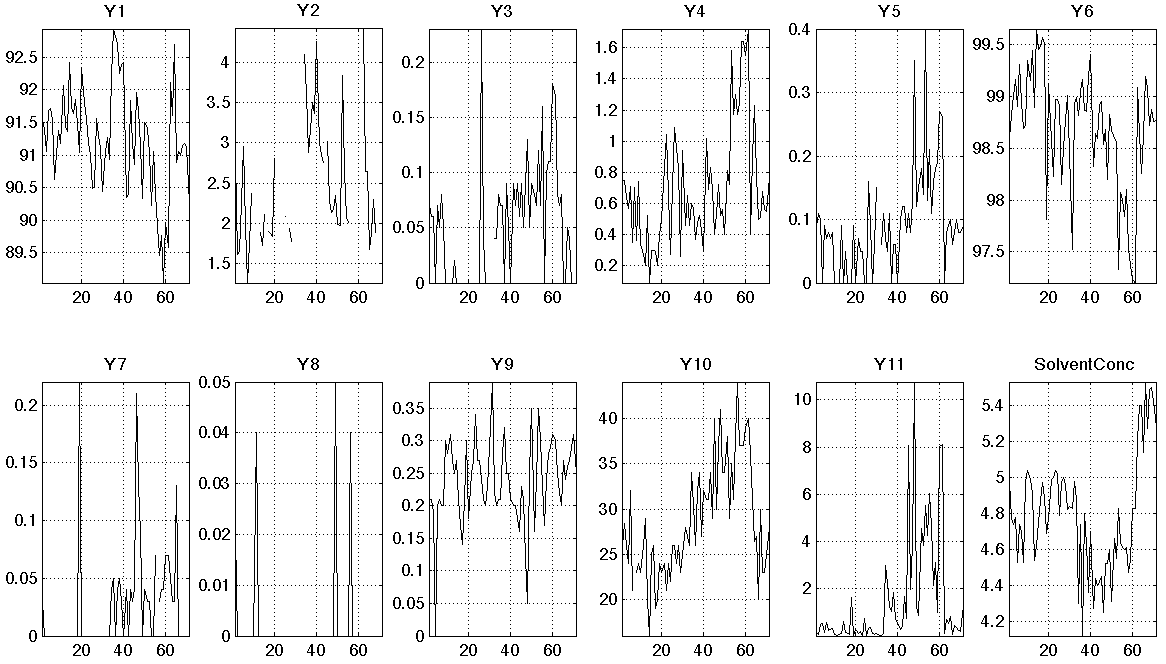
\includegraphics[width=\textwidth]{images/fmc/fmc-Z-raw-data.png}
\end{center}

\end{frame}

\begin{frame}\frametitle{About the batch trajectories}

\begin{itemize}
	\item	10 trajectories measured online
	
	\item	1 trajectory is the ``alignment time'' (shrink/stretch factor)
	
	\begin{center}
		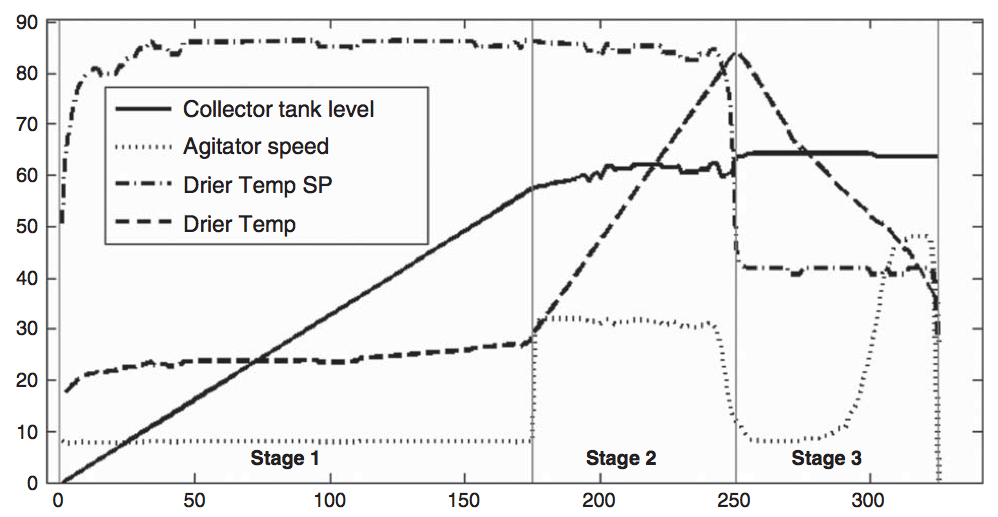
\includegraphics[width=\textwidth]{images/fmc/fmc-phases-4-trajectories.png}
	\end{center}	
	
\end{itemize}
\end{frame}

\begin{frame}\frametitle{About the initial conditions, \( \mathbf{Z}\)}

\begin{itemize}
	\item	Initial chemical analysis
	
	\item	Weight of wet cake
\end{itemize}

\end{frame}

\begin{frame}\frametitle{Feature-based approached}

What we learned from VIPs

\end{frame}

\begin{frame}\frametitle{Feature-based approached}

	\begin{itemize}
		\item	Alignment
		\item	Before and after shots
	\end{itemize}


\end{frame}
